\chapter{Introduction}
\label{ch:intro}

%    Move 1 establish your territory (say what the topic is about)
%    Move 2 establish a niche (show why there needs to be further research on your topic)
%    Move 3 introduce the current research (make hypotheses; state the research questions)


%    state the general topic and give some background
%    provide a review of the literature related to the topic
%    define the terms and scope of the topic
%    outline the current situation
%    evaluate the current situation (advantages/ disadvantages) and identify the gap
%    identify the importance of the proposed research
%    state the research problem/ questions
%    state the research aims and/or research objectives
%    state the hypotheses
%    outline the order of information in the thesis
%    outline the methodology

% https://www.scribbr.com/theses-examples/examples-dissertation-phd-theses/


\section{The pursuit of quantitative microscopy}

Methods for extracting quantitative information from microscopy
images typically rely on heuristic models intended to emulate
the perception of vision.
These heuristics identify regions of contrast as features
of interest and employ various image analysis techniques to estimate
the position, shape, and cross-sectional area of objects in the
field of view \cite{jahne97,gonzalez06,castleman96,pratt16,jain89}.
The field of quantitative microscopy has advanced recently with the
introduction of techniques that model the physics of image formation
to extract maximal quantitative information
from microscopic images \cite{lee07,bierbaum2017}.
This thesis describes advances in holographic particle characterization (HPC),
a microscopy technique for measuring
the three-dimensional position, size, and refractive index of
colloidal particles \emph{in situ}.

This work develops a formal foundation for the technique both by
advancing the theory of image formation in holographic microscopy
and also by reporting a suite of validation measurements
that establish the limits of precision and accuracy that can be
obtained with holographic video microscopy. In challenging
the assumptions inherent to the technique, we also introduce the
effective sphere model as a first-order model for
light scattering by aspherical particles that yields useful
characterization data.
Furthermore we describe how to mitigate the computational complexities
of detecting, localizing, and analyzing holographic features by
applying machine-learning algorithms to each stage of the analysis.
Finally, we demonstrate a real-world application
of HPC for optimizing the synthesis of monodisperse
colloidal spheres with size control. A diagram depicting the organization
of this thesis is provided in Fig.~\ref{fig:intro}.

\section{Organization}

\begin{figure}
  \centering
  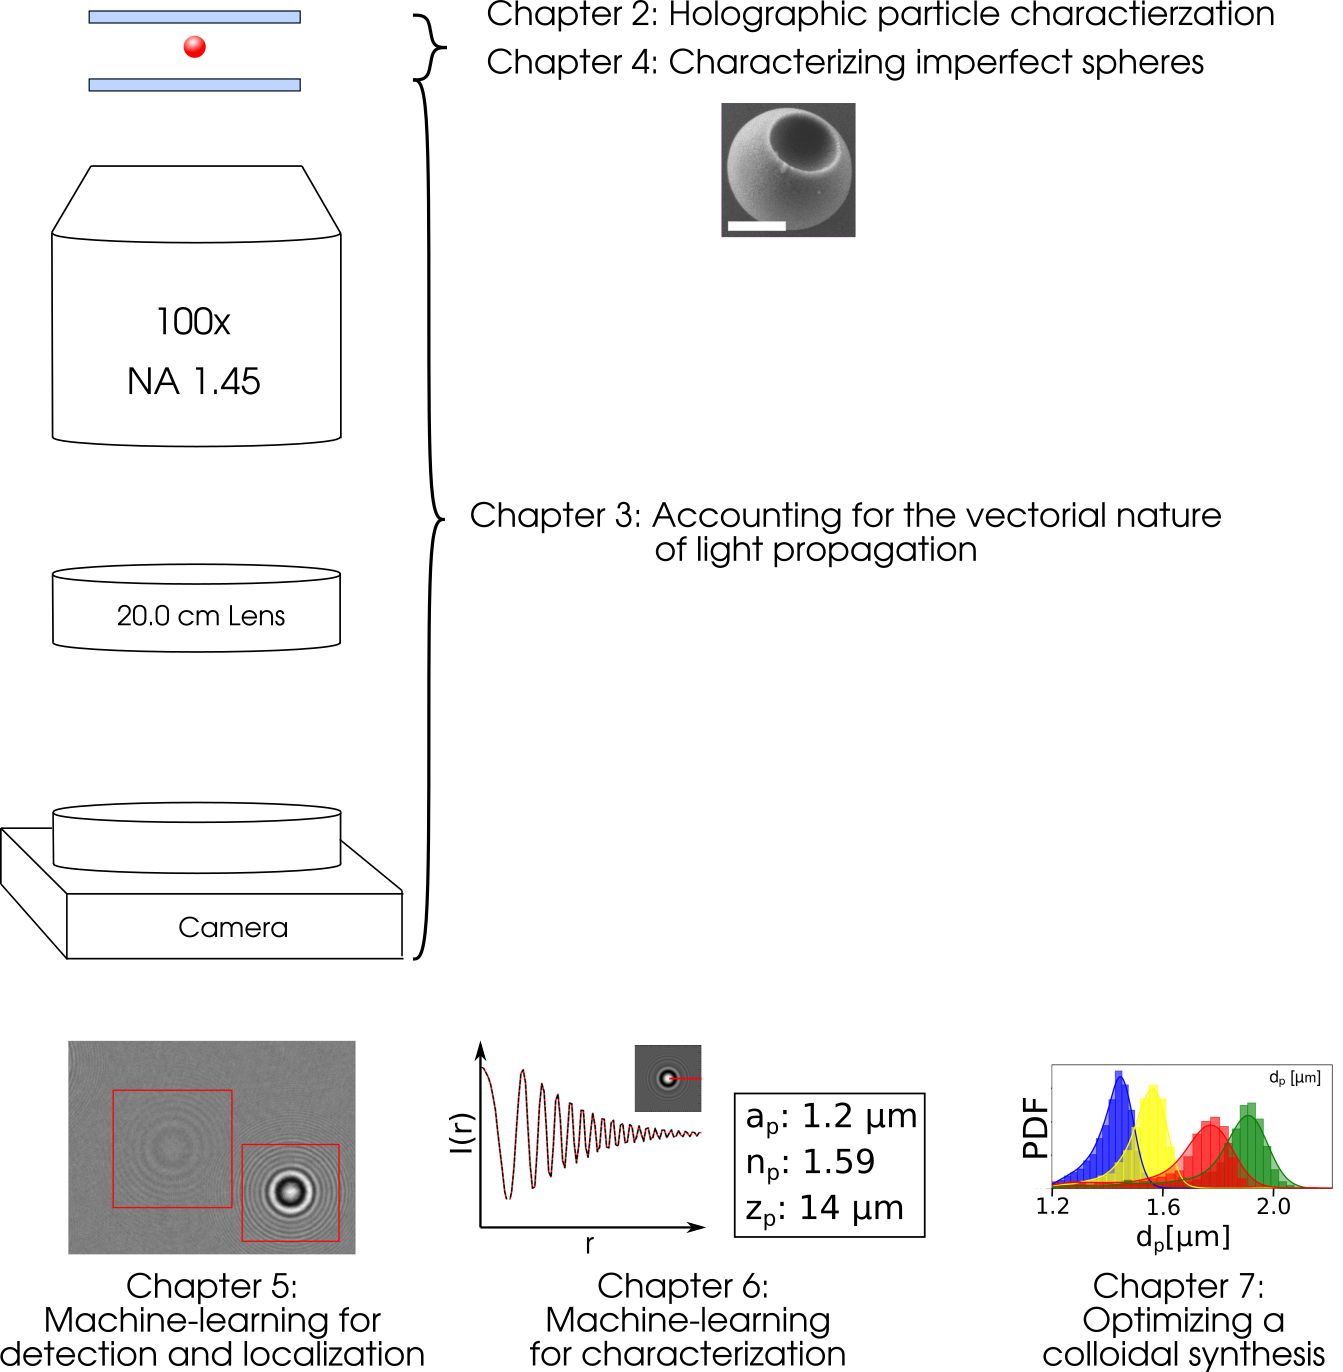
\includegraphics[width=\textwidth]{introduction_summary}
  \caption{Diagram summarizing the organization of this thesis.
    Chapters \ref{ch:hvm} and \ref{ch:dimpled} use a scalar
    theory of light scattering to characterize perfect and imperfect
    colloidal spheres. Chapter \ref{ch:debye} systematically
    accounts for the propagation of light through the optical
    train. Chapters \ref{ch:cascade} and \ref{ch:svr} improve
    image analysis with machine-learning algorithms for detection, localization,
    and characterization. Chapter \ref{ch:synthesis} demonstrates the use
    of holographic characterization for optimizing colloidal
    synthesis.}
  \label{fig:intro}
\end{figure}

\Autoref{ch:hvm} provides an extensive theoretical and practical
introduction to holographic particle characterization. The primary
experimental setup for all subsequent experiments is introduced and
a set of best practices are proposed for precision measurements. 

In \autoref{ch:debye}, we model the optical train to establish the
physical limits of HPC that are set by the imaging apparatus. The scattered
field and incident field are evaluated at several planes along the
optical train. The refraction of rays through each optical element
may impart a phase shift, a polarization rotation, and a scaling
of complex magnitude. We determine that a scalar theory
approximation successful accounts for the images arriving in the
focal plane for the domain of parameters we are interested in.

\Autoref{ch:dimpled} presents a series of experimental studies and
simulations that describe the effectiveness of Lorenz-Mie
microscopy for characterizing slightly aspherical particles.
Specifically, we synthesize and characterize three types of colloidal
particles: spheres, spheres will small dimples, and spheres with large dimples.
This study validates the use of the Lorenz-Mie theory
for analyzing spheres which have small deviations from
ideal sphericity and sets the stage for the effective-sphere model.

The first step in holographic particle characterization
requires detecting and localizing holographic features in experimental
images. Heuristic algorithms perform admirably for isolated, homogeneous
features; after tuning the necessary empirical parameters, they achieve
sub-pixel localization while incurring few false positives. Their
performance deteriorates, however, when they are presented with overlapping
features or with heterogeneous samples whose particles have disparate
characteristics. We present in \autoref{ch:cascade} two machine-learning
algorithms for detecting and localizing holographic features: a convolution
neural network (CNN) and a cascade classifier. Direct comparison with the
heuristic algorithm over a range of experimental and synthetic images
shows promising results. The CNN demonstrates robust feature detection
for overlapping holograms or even heterogeneous holographic features
in the same image and extends the domain of HPC to more dense, heterogeneous
samples. The cascade classifier's localization precision
is ten times worse than the CNN, but is also ten times faster than
the CNN. We show that the cascade classifier is fast enough for real-time
applications such as high-speed targeting in holographic optical
trapping systems.

After a holographic feature has been detected, initial estimates of the
scatter's size, refractive index, and three-dimensional position
are necessary for subsequent fitting to the Lorenz-Mie theory.
For homogeneous samples of a single particle type, the fitting procedure
can be initialized with a priori information. For heterogeneous samples
with disparate sizes or refractive indices, the fitting procedure
will likely lock onto local minima and return erroneous results for
the size and refractive index.
In \autoref{ch:svr} we demonstrate the use of a support vector machine for
estimating the size, refractive index, and axial displacement of scatterers
from holographic snapshots. Most holographic features subtend \SI{40000}{} pixels;
we reduce the dimensionality of each feature by averaging over the polar
angle to return the radial profile. In addition we produce a separate SVM to
estimate the size, refractive index, and height above the focal plane.
We demonstrate these support vector machines can rapidly resolve heterogeneous
samples with four greatly differing particle properties.

In the previous chapters we have worked towards validating and extending
the domain of applicability of holographic particle characterization.
In \autoref{ch:synthesis}, we close with a demonstration of its use for
optimizing the synthesis of 3-(trimethoxysilyl)propyl methacrylate (TPM)
colloidal spheres. The synthesis is principally a two-step procedure:
an emulsion of monodisperse, micrometer sized TPM droplets is prepared
and then polymerized. A number of experimental parameters and conditions
can however affect the resulting size of the polymerized spheres. In this
chapter we use holographic particle characterization to analyze
liquid droplets and solid TPM spheres. By synthesizing particles under a
number of differing protocols, we isolate a number of experimental conditions
that affect particle size.
